% - MTSA
%     Herramienta, sintaxis
% - Tests 
%     Qué tests desarrollamos, quizás mostrar un par interesantes y explicarlos

El algoritmo fue implementado en el lenguaje Java, agregando a la funcionalidad del programa Modal Transition System Analyser (MTSA)\cite{mtsaRepo}.

\section{MTSA}
El software utilizado cuenta con una gran cantidad de funcionalidad. Principalmente nos interesa la forma de escribir Labelled Transition Systems (LTS), esto se puede hacer mediante Finite State Process (FSP). En el listing~\ref{ejLTS} volvemos al caso de estudio presentado en~\ref{chpt:casoAviones} esta vez escrito en la herrmienta MTSA.

En primer lugar definimos las constantes que determinan la cantidad de sub-servicios a contratar. Luego definimos la componente \texttt{Agencia}, con un único estado que vuelve a sí mismo con las siguientes transiciones: \texttt{cancelacion, compra, query[servicio]}, este último se lee como cualquier transición \texttt{query[i]} si $i \in Servicio$.

Con la definición de los sub-servicios se puede ver una definición genérica compacta de múltiples componentes idénticas del problema, tantas como elementos haya en \texttt{Servicio}, cada una con su \texttt{id}, comenzado en 0, que es utilizado para definir transiciones únicas para cada componente. También se ve que para un componente más complejo simplemente se declaran más estados, cada uno con su nombre en mayúscula, sin necesidad de aclarar que pertenecen a un componente. Si se quiere que un estado tenga 2 transiciones que lleven a estados distintos se logra con el operador \texttt{|} (como ejemplo, ver el estado \texttt{Queried}).

Finalmente mostramos cómo se pueden componer las distintas LTSs con el comando \texttt{||}, con el cual nuestra planta compuesta tendrá tanto a la agencia como a los subservicios.

\begin{lstlisting}[language = mtsa, caption=Ejemplo de LTS y composición, label=ejLTS]
const N = 1
range Servicio = 0..(N-1)

Agencia = (
{cancelacion,compra} -> Agencia |
query[servicio] -> Agencia ).

SubService(id=0) = Unqueried,
Unqueried = (cancelacion -> Unqueried |
query[id] -> Queried),
Queried = (valido -> Disponible | noValido -> Imposible),
Disponible = ({compra,cancelacion} -> Unqueried),
Imposible = (canelacion -> Unqueried).

||Plant = Agencia || SubService[Servicio].
...
\end{lstlisting}

En el listing~\ref{ejController} vemos un ejemplo de cómo definir un controlador, en este caso lo llamamos $Goal$. En el área de \textit{Automated planning} el objetivo es alcanzar algún estado \textit{final}, es decir, los estados son los marcados; sin embargo en el contexto MTSA y al representar el problema con LTSs solo podemos marcar transiciones. La interpretación final es que las transiciones señaladas como \textit{marcadas} llevan a estados marcados y estos serán nuestros objetivos. En el ejemplo se declara la transición $compra$ como marcada, señalando la compra sin errores de un paquete. En este punto aclaramos, únicamente para facilitar cualquier intento de reproducción, que al utilizar transiciones marcadas, se puede generar un desdoblamiento de los estados. Como ejemplo notar que el estado \texttt{Agencia} va a tener (internamente) para la herramienta 2 versiones, una marcada alcanzada por $compra$ y otra no marcada alcanzada por $cancelacion$ y $query[servicio]$.

Luego definimos el conjunto de transiciones controlables, en este caso $cancelacion, compra$ y $ query[Servicio]$. Por último debemos agregar la palabra clave \texttt{nonblocking}, en caso contrario se intentará, por defecto, resolver otro problema de control fuera del alcance de este trabajo.

En la última línea utilizamos la palabra clave \texttt{heuristic} para aclarar que queremos utilizar el algoritmo de DCS, luego nombramos como $DirectedController$ al controlador que devuelve nuestro algoritmo cuando lo definimos como el LTS $Compuesto$ ($Plant$)\footnote{Cabe destacar que a esta altura la composición todavía no fue calculada} que cumple con la especificación $Goal$.

\begin{lstlisting}[language = mtsa, caption=Ejemplo de Controller y DCS, label=ejController]
...
controllerSpec Goal = {
marking = {compra}
controllable = {cancelacion, compra, query[Servicio]}
nonblocking
}

heuristic ||DirectedController = Plant~{Goal}.
\end{lstlisting}

\section{Heurísticas adicionales}\label{chpt:heurist-nuevas}
\subsection{Dummy/Debugging}
Como dijimos en el capítulo \ref{chpt:background}, el algoritmo de DCS debe ser agnóstico a la heurística. Al comenzar nuestro trabajo en el proyecto y una vez que pudimos generar cierto conocimiento sobre el pseudocódigo existente nos percatamos de casos borde que no iban a ser bien resueltos. Sin embargo, al correr dichos casos el resultado era correcto, esto se debía a que la heurística era muy buena y lograba ir por un camino directo al Goal (o Error, depende el caso); entonces no caía en nuestra ``trampa''.

En función de poner a prueba sólo el algoritmo de exploración desarrollamos una heurística de debugging o \textit{Dummy}. La misma ordena las transiciones a explorar alfabéticamente, dejando primero las no controlables pero sin mirar información sobre distancia a marcados o error. Decidimos dejar el ordenamiento de no controlables primero ya que esto no es heurístico, se sabe por especificación qué transiciones son controlables y cuáles no.

A partir de entonces usamos los nombres de las transiciones para explorar nuestros casos de test de la forma que nos interesaba, ganando así control sobre los tests.

\subsection{BFS}
Si bien el algoritmo debe ser agnóstico a la heurística, la misma puede (y seguramente lo haga) modificar los tiempos de ejecución. Ya que si llega antes a alguna conclusión sobre un estado ésta información se puede propagar, cortando más ramas y/o más grandes.

La segunda heurística que desarrollamos es un simple BFS. La razón es para mostrar qué tanto se pueden mejorar los tiempos del algoritmo con una buena heurística. Esto se puede ver en detalle en el capítulo \ref{chpt:performance}, donde mostramos resultados de un mismo benchmark para las diferentes heurísticas.

\section{Testing}
Luego de haber mostrado la sintaxis con la cual desarrollamos nuestros tests vamos a hablar un poco de ellos y detalles sobre algunos a destacar. El listing \ref{ejTest1} muestra un ejemplo de sintaxis completo (test 1). Si se desea ver la especificación de cada uno de los tests puede encontrarse en el repositorio de MTSA\footnote{\href{https://bitbucket.org/lnahabedian/mtsa/src/master/maven-root/mtsa/src/test/resources/NonBlocking/}{https://bitbucket.org/lnahabedian/mtsa/src/master/maven-root/mtsa/src/test/resources/NonBlocking/}}.

\begin{lstlisting}[language = mtsa, caption=Test 1 a modo de ejemplo, label=ejTest1] 
Ejemplo = A1,
A1 = (u12 -> A2 | u14 ->A4),
A2 = (u21 -> A1),
A4 = (c45 ->A5),
A5 = (u55 -> A5).

||Plant = Ejemplo.

controllerSpec Goal = {
controllable = {c45}
marking = {u55}
nonblocking
}

heuristic ||C = Plant~{Goal}.
\end{lstlisting}

En total tenemos una batería de \totalTests\ tests. Los cuales no fueron desarrollados uno detrás del otro sino que utilizamos una técnica llamada TDD (Test Driven Development). Desde el pseudocódigo e implementación existente de DCS iniciamos la batería de tests con algunos casos borde que resolvía mal.
Luego entramos en un ciclo donde fuimos generando versiones que corregían los casos y más tests que rompían otras partes del algoritmo. Además en ciertos puntos críticos decidimos refactorizar completamente partes amplias de la implementación, fuera de las refactorizaciones chicas al pasar los tests.

Dentro de la batería queremos destacar algunos de especial interés, agrupados según qué problema específico atacan. Antes necesitamos explicar un poco de notación, las transiciones empezadas con $u$/$c$ son no-controlables/controlables respectivamente, los estados marcados son los que tienen doble borde; en ciertos tests con transiciones nombradas diferente vamos a aclarar en la explicación cuáles son las controlables.
\bigskip

\FloatBarrier
%-----------------------------------------------------------------------------------------------
\subsection{Marcado explícito de errores}\label{marcarErrores}

% FALENCIAS AL ENCONTRAR ERRORES
Un estado deadlock (sin transiciones de salida) es obviamente un error, ya que si caemos en él no podemos alcanzar nunca un estado marcado. Ahora, ¿qué pasa si tenemos un conjunto de estados conectados entre sí pero sin conexión a otros fuera del conjunto?. Depende de si existe un estado marcado dentro del conjunto o no, ya que de no haberlo no tenemos forma de alcanzar uno (no podemos salir del conjunto). 

La figura \ref{fig:falenciasErrores} ejemplifica este caso, el conjunto o rama $B$ fue totalmente explorado y no contiene ningún estado marcado. En este momento es importante que agreguemos todos los estados de $B$ a $\Errors$, de no hacerlo podríamos incurrir en una falla al propagar goal desde otra rama. Es decir, si se mira primero la rama de abajo y no lo marcamos como error (a pesar de estar completamente explorado), entonces al mirar la de arriba diremos que es goal y propagaremos dicha información, equivocadamente, más allá de $e$. 

Éste problema se evita respetando el invariante presentado en la propiedad \ref{def:invariant}, ya que si una rama $B$ cuya raíz es $s$ está totalmente explorada, entonces $E_s \subseteq E$ es la reducción del problema que decide si $s$ es un estado ganador o perdedor. Además, como está totalmente explorada $\unexploredToBottom{E_s} = \unexploredToTop{E_s}$, por lo que $W_{\unexploredToBottom{E_s}} \cup L_{\unexploredToTop{E_s}} = S_{E_{s}}$ y no puede darse el caso de la figura \ref{fig:falenciasErrores} en el que los estados de la rama no fueron clasificados.

\begin{figure}[htb]
	\centering
	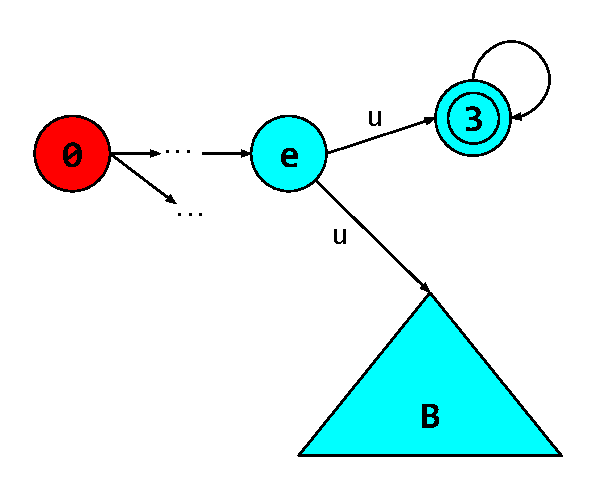
\includegraphics[width=\linewidth/2]{figures/FalenciasErrores.pdf}
	\caption{Caso sub-autómata completamente explorado (B), sin marcados dentro.}
	\label{fig:falenciasErrores}
\end{figure}

\FloatBarrier
\textbf{Test 8} Fig \ref{fig:test8} 
Este es un caso muy similar al presentado como ejemplo pero en lugar de una rama perdedora (llamada B) totalmente explorada a partir de u23 tenemos un solo estado (3). Si no se señala el estado 3 como error, porque no se detecta que es un livelock, entonces podríamos sacar la conclusión errada de que la planta es controlable; ya que 2 forma un loop con el estado inicial marcado. Los livelocks y las ramas perdedoras son difíciles de detectar hasta ser totalmente exploradas, pero en ese momento deben ser categorizados como errores, de otra forma no pueden distinguirse las ramas ya confirmadas como error y las parcialmente exploradas. Una vez que el estado 3 es marcado como error, concluir que la planta no es controlable resulta sencillo.

\begin{figure}[h]
 \centering
 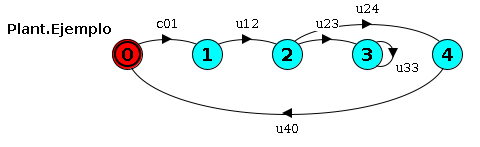
\includegraphics[scale=0.7]{figures/tests/test8.png}
 \caption{LTS del test 8}
 \label{fig:test8}
\end{figure}

\FloatBarrier
\textbf{Test 12} Fig \ref{fig:test12}
Variante del test 8, en este caso existe controlador ya que los estados [0,3,4,5] forman un loop con un estado marcado, y puede desactivarse $c\_0\_m1$ para evitar salir del loop. Notar que aunque el estado 1 esté marcado es necesario dejarlo fuera del controlador para poder asegurar la victoria, ya que si se alcanza el estado 1 no puede evitarse una extensión al estado 2, el cual es perdedor. Notar que con extenderse para llegar a un estado marcado es suficiente, no es necesario alcanzarlos a todos.
\begin{figure}[h]
 \centering
 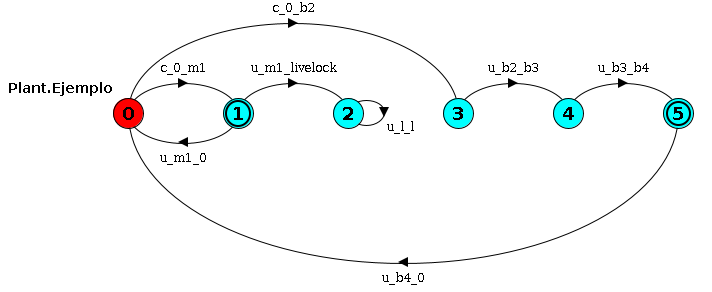
\includegraphics[scale=0.6]{figures/tests/test12.png}
 \caption{LTS del test 12}
 \label{fig:test12}
\end{figure}

\FloatBarrier
%-----------------------------------------------------------------------------------------------
\subsection{Propagación local vs por conjuntos}\label{propagacionLocal}

% PROPAGACION LOCAL
Una vez obtenido un resultado necesitamos propagarlo hacia los estados ancestros. Necesitamos saber, para cada estado, si es posible sacar una conclusión dada la nueva información. Muchas veces es imposible hacerlo teniendo una mirada local, analizando solo un estado a la vez, ya que se pierde información sobre lo que sucede dentro del ``conjunto'' de ancestros vecinos.

Por ejemplo en el caso de la figura \ref{fig:propagarError}, hay un loop controlable entre dos estados, el cual se explora primero, y uno de ellos va controlablemente a un error. Debe habilitarse alguna controlable saliente del estado 2 (caso contrario sería un deadlock), pero ninguna lleva a un estado ganador, por ende la planta es no controlable. Sin embargo, según la mirada local nunca se concluiría que los estados [1, 2] son errores, porque ambos tienen \textit{una forma de escapar del error}, el otro estado del loop, y no se sabe que ese otro estado está en la misma situación. 

Equivalentemente la mirada local tampoco funciona propagando $\Goals$, en la figura \ref{fig:propagarGoal} se puede ver un ejemplo. El estado $2$ llega al estado marcado $3$ pero no puede forzarlo, sin importar si la transición a $3$ es controlable o no ya que tiene una transición no controlable a $1$. Como $1$ solo puede volver a $2$ ésta situación no nos molestaría (por ser non-blocking) y el modelo debería ser controlable. Ahora si miramos localmente al propagar $Goal$ desde $3$ \textit{no sabemos dónde nos lleva la transición no controlable de 2 a 1}, y deberíamos suponer lo peor, sin poder marcar a 2 como ganador.

Entonces una mirada local no funciona a la hora de propagar. Pero ¿qué conjunto de ancestros vecinos deberíamos tomar? Es difícil decidir dónde hacer el corte; son muchos casos y no se puede, localmente, distinguirlos a todos. Por ende es necesario una propagación más inteligente, con una mirada global del conjunto de ancestros.

Como se detalló en el capítulo \ref{chpt:dcs}, al momento de propagar resultados recurrimos a un punto fijo, tanto para $\Goals$ como $\Errors$. De esta forma tenemos en cuenta toda la información acumulada de los estados en cuestión. Si bien esto implica un mayor costo de cómputo, asegura la correcta propagación de información, lo que más adelante facilita, por ejemplo, la detección de ciclos perdedores.\\

\begin{figure}[htb]
	\centering
	\makebox[\linewidth][c]{%
		\begin{subfigure}[t]{.5\textwidth}
			\centering
			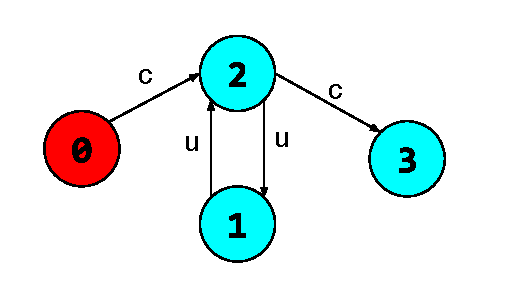
\includegraphics[width=\linewidth]{figures/PropagarError.pdf}  
			\caption{Propagar errores}
			\label{fig:propagarError}
		\end{subfigure}
		\begin{subfigure}[t]{.5\textwidth}
			\centering
			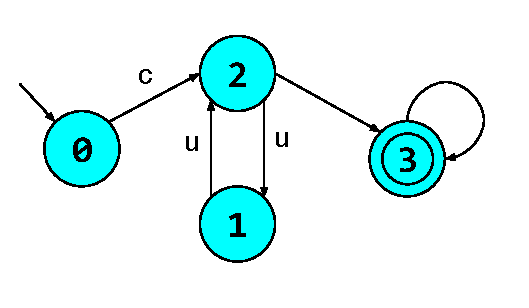
\includegraphics[width=\linewidth]{figures/PropagarGoal.pdf}  
			\caption{Propagar goals}
			\label{fig:propagarGoal}
		\end{subfigure}
	}
	\caption{Problemas de propagación local.}
	\label{fig:propagacionLocal}
\end{figure}

\textbf{Test 1} Fig \ref{fig:test1}
En este test, al descubrir que el estado 2 es ganador y propagar esa información, debe decidirse si el estado 0 es ganador. En principio parecería que no, puesto que un evento no controlable puede forzarlo a 3, pero es necesario darse cuenta que, si bien 0 puede ser forzado a 3, luego está obligado a volver, por lo que siempre hay una extensión que alcanza a 2. Por ende existe un director, que es el mismo autómata.
\begin{figure}[h]
 \centering
 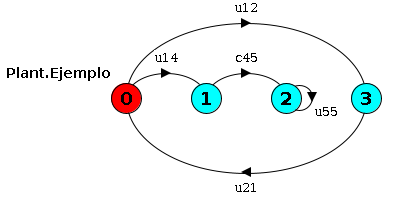
\includegraphics[scale=0.7]{figures/tests/test1.png}
 \caption{LTS del test 1}
 \label{fig:test1}
\end{figure}


\FloatBarrier
\textbf{Test 26} Fig \ref{fig:test26} 
El loop [2,3,4] es ganador, pero desde el estado 2 el ambiente puede no controlablemente tomar el evento $u20$ para llegar al estado 0 y escapar al loop. La clave es que desde [0,1,2] siempre puede alcanzarse el mismo estado marcado 4, en realidad toda la planta es una componente fuertemente conexa con un estado marcado y por lo tanto es controlable. 
Si la propagación fuera local viendo un estado a la vez, concluiríamos que el estado 2 no puede marcarse como ganador porque un evento no controlable lo puede forzar al estado 0, el cual no sabemos si es perdedor.

\begin{figure}[h]
 \centering
 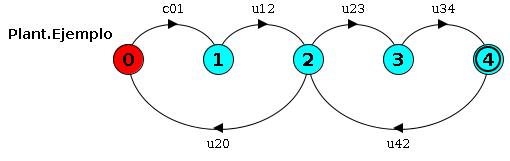
\includegraphics[scale=0.7]{figures/tests/test26.png}
 \caption{LTS del test 26}
 \label{fig:test26}
\end{figure}

\FloatBarrier
%-----------------------------------------------------------------------------------------------
\subsection{Correcta detección de loops ganadores}

La detección de loops con estados ganadores es una pieza central para la optimización y corrección del algoritmo, y tampoco puede solucionarse con una mirada local. Es sencillo dar una descripción declarativa de los estados a encontrar (ver listing \ref{lst:viejoMCCC}) pero no resulta claro cómo implementarla. 

Luego de varios intentos más performantes pero que presentaban fallas, llegamos a la conclusión de utilizar un algoritmo de punto fijo clásico (similar a listing \ref{lst:classical}) pero con una planta reducida. Los enfoques más veloces que intentamos sí funcionaron a la hora de detectar errores y terminaron sembrando las bases para \texttt{findNewErrorsIn($loops$)}.

Como se vió en el capítulo \ref{chpt:dcs}, para detectar ganadores corremos un algoritmo clásico sobre una versión pesimista de la planta explorada, asumiendo que toda transición no vista es perdedora. Además solo tomamos en cuenta un grupo reducido, de los estados ya explorados, que forma un loop sobre la última transición expandida. Este enfoque otorga la completitud del algoritmo tradicional sosteniendo la eficiencia de la exploración on-the-fly.

\begin{lstlisting}[language={pseudocode},label={lst:viejoMCCC},caption={vieja descripción estados ganadores},float=ht, frame=single]
function buildMCCC($e, e'$):
let $C$ such that
$C = \{ e_i \mid (e' \runw{w}{\structure} e_i \runw{w'}{\structure} e \vee e \runw{w}{\structure} e_i \runw{w'}{\structure} e') \wedge $extendsCCC($e_i,C \cup \Goals$)$ \wedge$
$(\exists w \ldot e \runw{w}{\structure} e_m \wedge e_m \in M_E \cap (C \cup \Goals)) \}$
return $C$

function extendsCCC($e, C$):
return $(\exists \l \ldot e \step{\l}{E} e' \wedge e' \in C) \wedge (\forall \l_u \in A_U \ldot e \step{\l_u}{E} e' \Rightarrow e' \in C)$

\end{lstlisting}

\FloatBarrier
\textbf{Test 35} Fig \ref{fig:test35} 
Este test utiliza la heurística debugging y su funcionalidad de ordenar las transiciones alfabéticamente. Las transiciones controlables son \{e, a, i\}; recordar que los eventos no-controlables se exploran primero.

A la hora de armar por punto fijo un conjunto de estados ganadores hay que tener mucho cuidado de no quedarse sin estados marcados o a un paso de goal, ya que estos son los que le dan la capacidad de ganar al conjunto (ver función \texttt{findNewGoalsIn} en el listing \ref{lst:dcs.gather}). El test 35 resalta esta problemática al analizar el loop [2,3,4,5,6], como el evento $f$ es no controlable y el estado 5 es un livelock, la función \texttt{findNewGoalsIn} remueve al estado 4 del conjunto a analizar. Esto causa que el estado 2 sea inalcanzable por los estados restantes del conjunto, y también es removido; pero como $e$ es controlable todavía tenemos un conjunto controlablemente cerrado [3,6] que se querría marcar como ganadores. Aquí podría terminar el punto fijo, pero debe tenerse cuidado en que en el conjunto resultante todavía haya estados marcados (o a un paso de goal) a los cuales alcanzar, cosa que no ocurre en este caso, por lo que ningún estado de [2,3,4,5,6] es ganador.

La correcta solución para esta planta es un controlador que desactiva el evento $a$ y es ganador por alcanzar el self loop del estado marcado 1.

\begin{figure}[h]
 \centering
 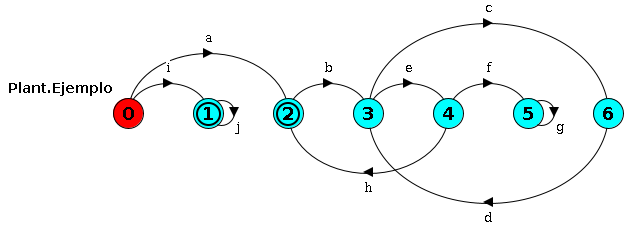
\includegraphics[scale=0.7]{figures/tests/test35.png}
 \caption{LTS del test 35}
 \label{fig:test35}
\end{figure}

\FloatBarrier
\textbf{Test 41} Fig \ref{fig:test41}
También se utiliza la heurística debugging, y la transición controlable es $a04c31$. 
La clave es que \texttt{findNewGoalsIn} debe detectar nuevos loops ganadores tanto si tienen un estado ganador a un paso como si contienen estados marcados. 
La heurística debugging es esencial para el test, porque queremos testear la detección de nuevos loops ganadores, no la propagación. El estado 2 es marcado como ganador antes de explorar $a03u23$ y cerrar el loop [0,1,3]. Esto evita que al propagar el goal del estado 2 se marque a los estados 0,1 y 3 como ganadores; porque no se sabe a donde lleva $a03u23$.
Luego, el conjunto [0,1,3] es ganador por tener un estado Goal a un paso (el estado $2$).

\begin{figure}[h]
 \centering
 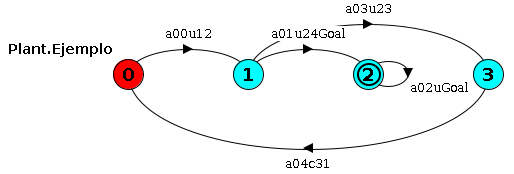
\includegraphics[scale=0.7]{figures/tests/test41.png}
 \caption{LTS del test 41}
 \label{fig:test41}
\end{figure}


\FloatBarrier
\textbf{Test 49} Fig \ref{fig:test49}
Es similar al test 35 pero en este caso no existe controlador. Luego de hacer el punto fijo en \texttt{findNewGoalsIn} para quedarse con los estados ganadores, puede quedar más de un componente fuertemente conexo de estados. En dicho caso solo los conjuntos que tengan marcados/ganadores a un paso son los que deberían ir a $\Goals$, ya que los estados de otros componentes no podrán llegar a ellos de manera segura. En particular \texttt{findNewGoalsIn} remueve los estados que no pueden alcanzar goals o marcados dentro del conjunto al final de cada iteración del punto fijo. Esto asegura que las componentes conexas incluyan un estado marcado o estén a un paso de un estado ya señalado como goal.

Concretamente lo que sucede al explorar la planta es que por el orden de la heurística debugging se van descubriendo los loops chicos, terminando de cerrar todo con la transición $u10$. En este momento se buscan ganadores dentro del loop [0, 1, 2, 3, 4, 5], como el estado 2 tiene una no-controlable por explorar ($u99$ se explora penúltima) es removido del conjunto dejando dos componentes conexas, [0, 1] y [3, 4, 5]. De no tener cuidado podríamos asumir que todos son goals ya que existe un marcado dentro del conjunto total [0, 1, 3, 4, 5]. Pero este (estado 5) no puede ser alcanzado de forma segura por la componente conexa [0, 1]. Por esto, se marca a los estados [3, 4, 5] como ganadores pero ya que el estado inicial 0 no puede alcanzar los estados ganadores sin pasar por 2 que es perdedor, la planta no es controlable.
\begin{figure}[h]
 \centering
 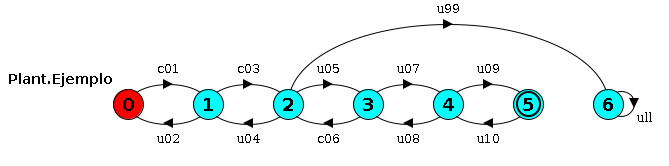
\includegraphics[scale=0.7]{figures/tests/test49.png}
 \caption{LTS del test 49}
 \label{fig:test49}
\end{figure}
